\clearpage
\section{Fixed task sets}
\label{app:fixed_populations}

A line that summarizes tasks (a mean, a median or a pooled agreement) against model size or training reads, at each point, the tasks that have a value there. The above-chance gate keeps more tasks at larger sizes and the three-pair minimum empties some cells, so a line can rise or fall because its tasks change. Each figure below redraws a paper figure with one task set per line, the tasks that have a value at every point of that line (solid), and draws the original line dashed behind it. Figure~\ref{fig:app_rq02_fixed_rq2} redraws Figure~\ref{fig:rq2}, Figure~\ref{fig:app_rq02_fixed_decision_accuracy} Figure~\ref{fig:app_rq02_decision_accuracy}, Figure~\ref{fig:app_rq05_fixed_design_decisions} Figure~\ref{fig:app_rq05_design_decisions}, Figure~\ref{fig:app_rq10_fixed_size_generalisation} Figure~\ref{fig:app_rq10_size_generalisation}, Figure~\ref{fig:app_rq11_fixed_evaluation_recipe} Figure~\ref{fig:app_rq11_evaluation_recipe}, Figure~\ref{fig:app_rq12_fixed_above_chance_items} Figure~\ref{fig:app_rq12_above_chance_items}, and Figure~\ref{fig:app_rq13_fixed_english_only} Figure~\ref{fig:app_rq13_english_only}.

\begin{figure*}[p]
\centering
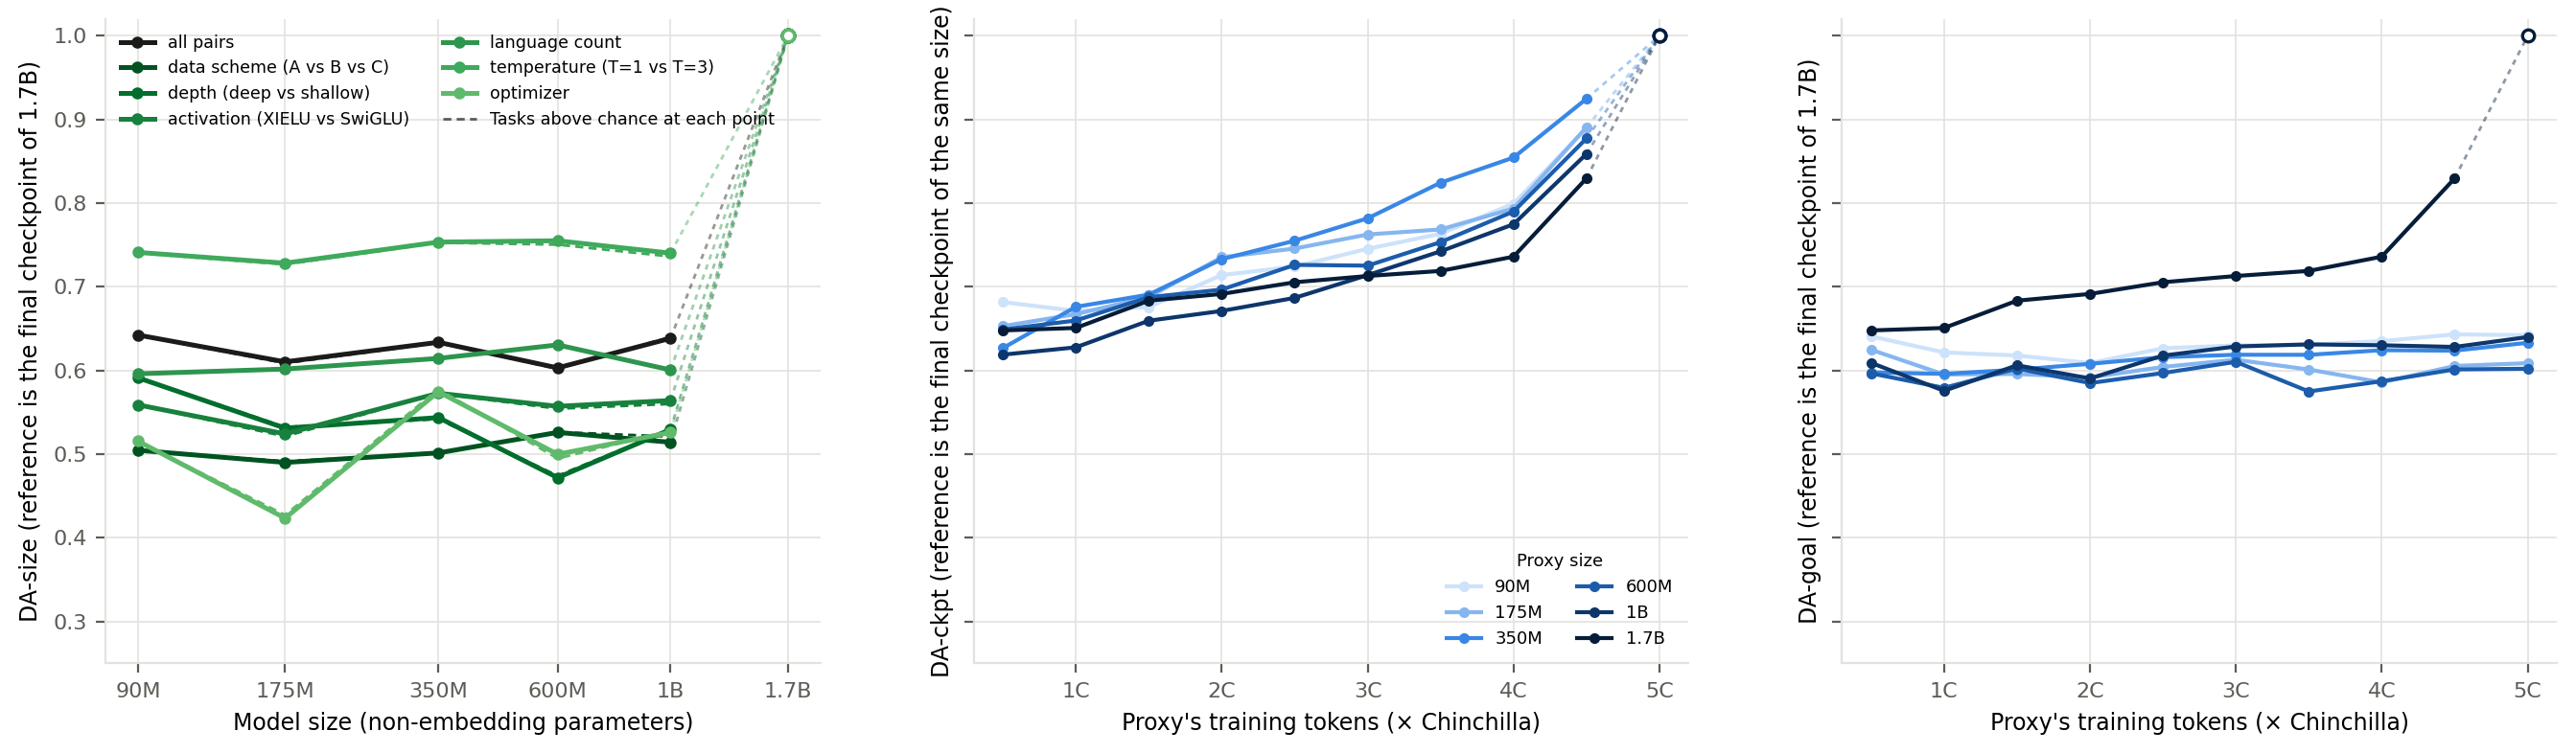
\includegraphics[width=\textwidth,height=0.8\textheight,keepaspectratio]{figures/app_rq02_fixed_rq2.png}
% source: src/signal-and-noise/analysis/rq02_decision_accuracy/pretraining/predictivity/rq2_da_all_above_66_either_transformation_mono_axis_fixed_tasks_paper.png
\caption{\textbf{Holding the tasks fixed moves the DA-size line over every single-axis pair by less than 0.01, small against the line's own range, so its shape is not a population effect.} Figure~\ref{fig:rq2} redrawn with one task set per line, the reliable tasks of each line that have a value at every point (solid), against the original (dashed). On the 702 tasks with a value at every point, the line reads 0.64 at 90M and 0.64 at 1B, against 0.64 and 0.64 on the tasks of each point (705--734). Over every line of the panel the largest shift is $-$0.01 (data scheme (A vs B vs C), at 1B).}
\label{fig:app_rq02_fixed_rq2}
\end{figure*}

\begin{figure*}[p]
\centering
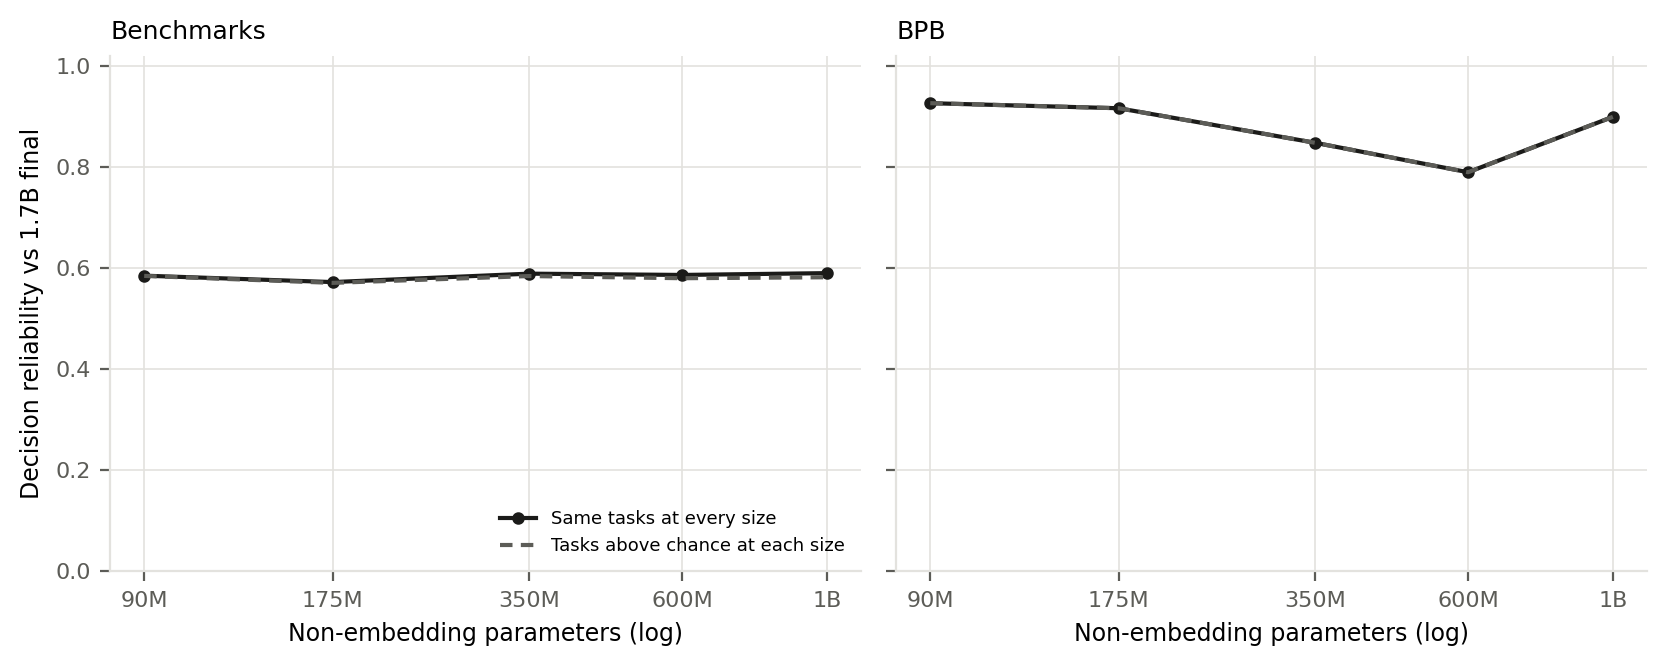
\includegraphics[width=\textwidth,height=0.8\textheight,keepaspectratio]{figures/app_rq02_fixed_decision_accuracy.png}
% source: src/signal-and-noise/analysis/rq02_decision_accuracy/pretraining/predictivity/scale_convergence_da_size_multi_axes_fixed_tasks_paper.png
\caption{\textbf{Holding the tasks fixed moves the benchmark line by at most +0.01 (at 1B), so part of the line's movement comes from its changing tasks.} Figure~\ref{fig:app_rq02_decision_accuracy} redrawn with one task set per line, the tasks above chance that have a value at every point (solid), against the original (dashed). On the 1267 tasks with a value at every point, the line reads 0.58 at 90M and 0.59 at 1B, against 0.58 and 0.58 on the tasks of each point (1274--1461).}
\label{fig:app_rq02_fixed_decision_accuracy}
\end{figure*}

\begin{figure*}[p]
\centering
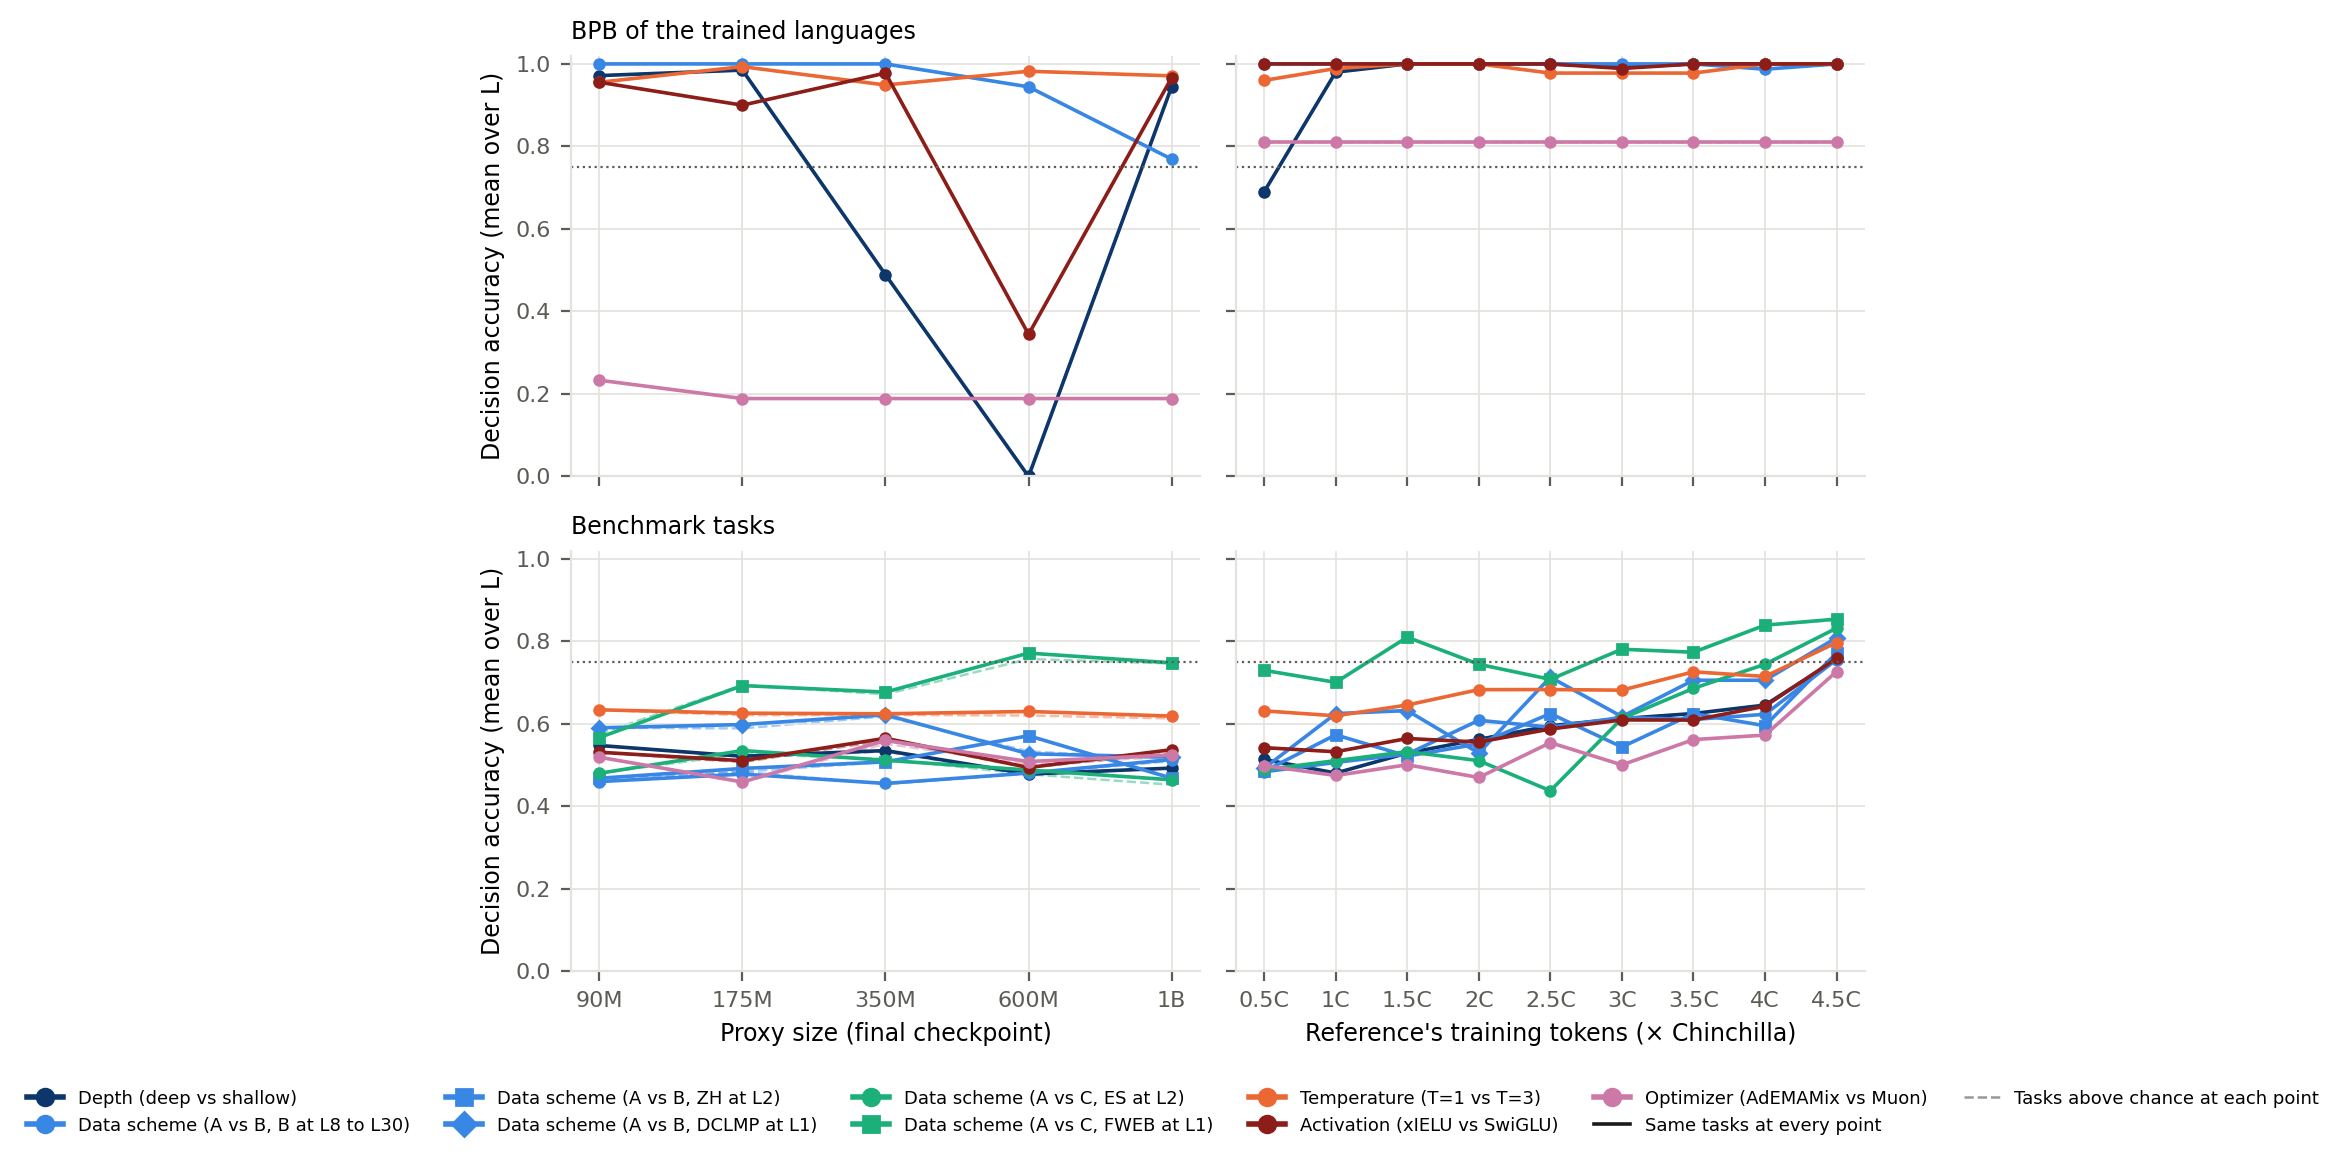
\includegraphics[width=\textwidth,height=0.8\textheight,keepaspectratio]{figures/app_rq05_fixed_design_decisions.png}
% source: src/signal-and-noise/analysis/rq05_design_decisions/pretraining/predictivity_seeds/da_all_lines_mono_axis_fixed_tasks_paper.png
\caption{\textbf{Holding the tasks fixed moves the benchmark line of the A vs DCLMP decision by at most +0.01 (at 175M), small against the line's own range, so its shape is not a population effect.} Figure~\ref{fig:app_rq05_design_decisions} redrawn with one task set per line, the (task, language setting) cells of each line that have a value at every point (solid), against the original (dashed). On the 127 cells with a value at every point, the line reads 0.59 at 90M and 0.52 at 1B, against 0.59 and 0.51 on the cells of each point (127--136). Over every line of the panel the largest shift is +0.01 (scheme\_C:FWEB / benchmark, at 600M).}
\label{fig:app_rq05_fixed_design_decisions}
\end{figure*}

\begin{figure*}[p]
\centering
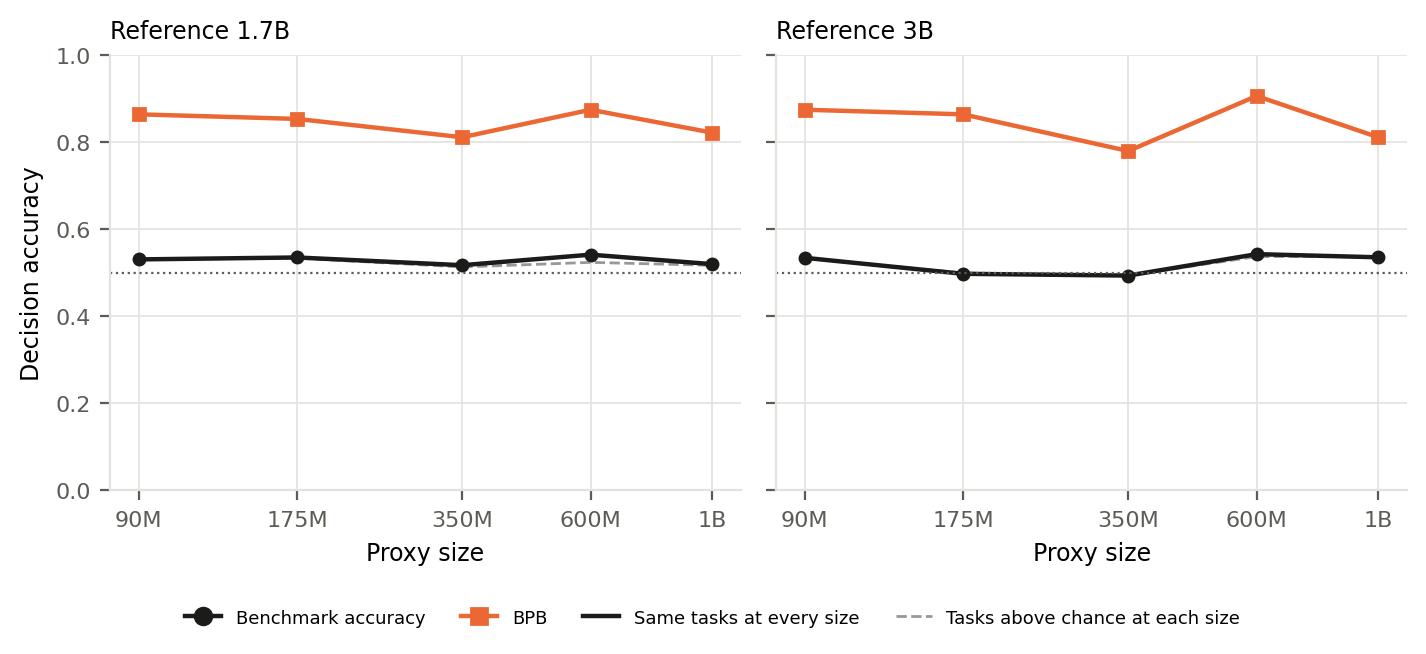
\includegraphics[width=\textwidth,height=0.8\textheight,keepaspectratio]{figures/app_rq10_fixed_size_generalisation.png}
% source: src/signal-and-noise/analysis/rq10_size_generalisation/pretraining/predictivity/gate_share_and_da_size_mono_axis_fixed_tasks_paper.png
\caption{\textbf{Holding the tasks fixed moves the benchmark line against the 3B reference by at most +0.01 (at 600M), small against the line's own range, so its shape is not a population effect.} Figure~\ref{fig:app_rq10_size_generalisation} redrawn with one task set per line, the tasks of each channel (the left panel is not redrawn) that have a value at every point (solid), against the original (dashed). On the 469 tasks with a value at every point, the line reads 0.53 at 90M and 0.54 at 1B, against 0.53 and 0.54 on the tasks of each point (471--568). Holding the tasks fixed moves the benchmark line against the 1.7B reference by at most +0.02 (at 600M), so part of the line's movement comes from its changing tasks.}
\label{fig:app_rq10_fixed_size_generalisation}
\end{figure*}

\begin{figure*}[p]
\centering
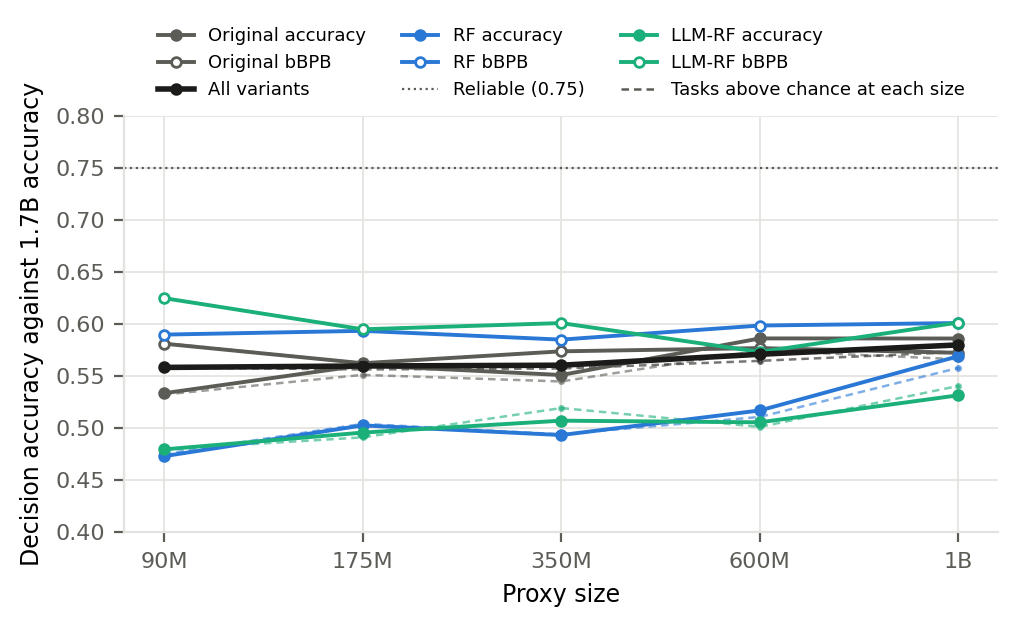
\includegraphics[width=\textwidth,height=0.8\textheight,keepaspectratio]{figures/app_rq11_fixed_evaluation_recipe.png}
% source: src/signal-and-noise/analysis/rq11_evaluation_recipe/pretraining/predictivity/recipe_da_size_variants_multi_axes_fixed_tasks_paper.png
\caption{\textbf{Holding the tasks fixed moves the pooled line by at most +0.01 (at 1B), so part of the line's movement comes from its changing tasks.} Figure~\ref{fig:app_rq11_evaluation_recipe} redrawn with one task set per line, the tasks of each variant that have a value at every point (solid), against the original (dashed). On the 943 tasks with a value at every point, the line reads 0.56 at 90M and 0.58 at 1B, against 0.56 and 0.57 on the tasks of each point (955--1142). Over every line of the panel the largest shift is +0.02 (Original accuracy, at 1B). Holding the tasks fixed moves the original accuracy line by at most +0.02 (at 1B), so part of the line's movement comes from its changing tasks.}
\label{fig:app_rq11_fixed_evaluation_recipe}
\end{figure*}

\begin{figure*}[p]
\centering
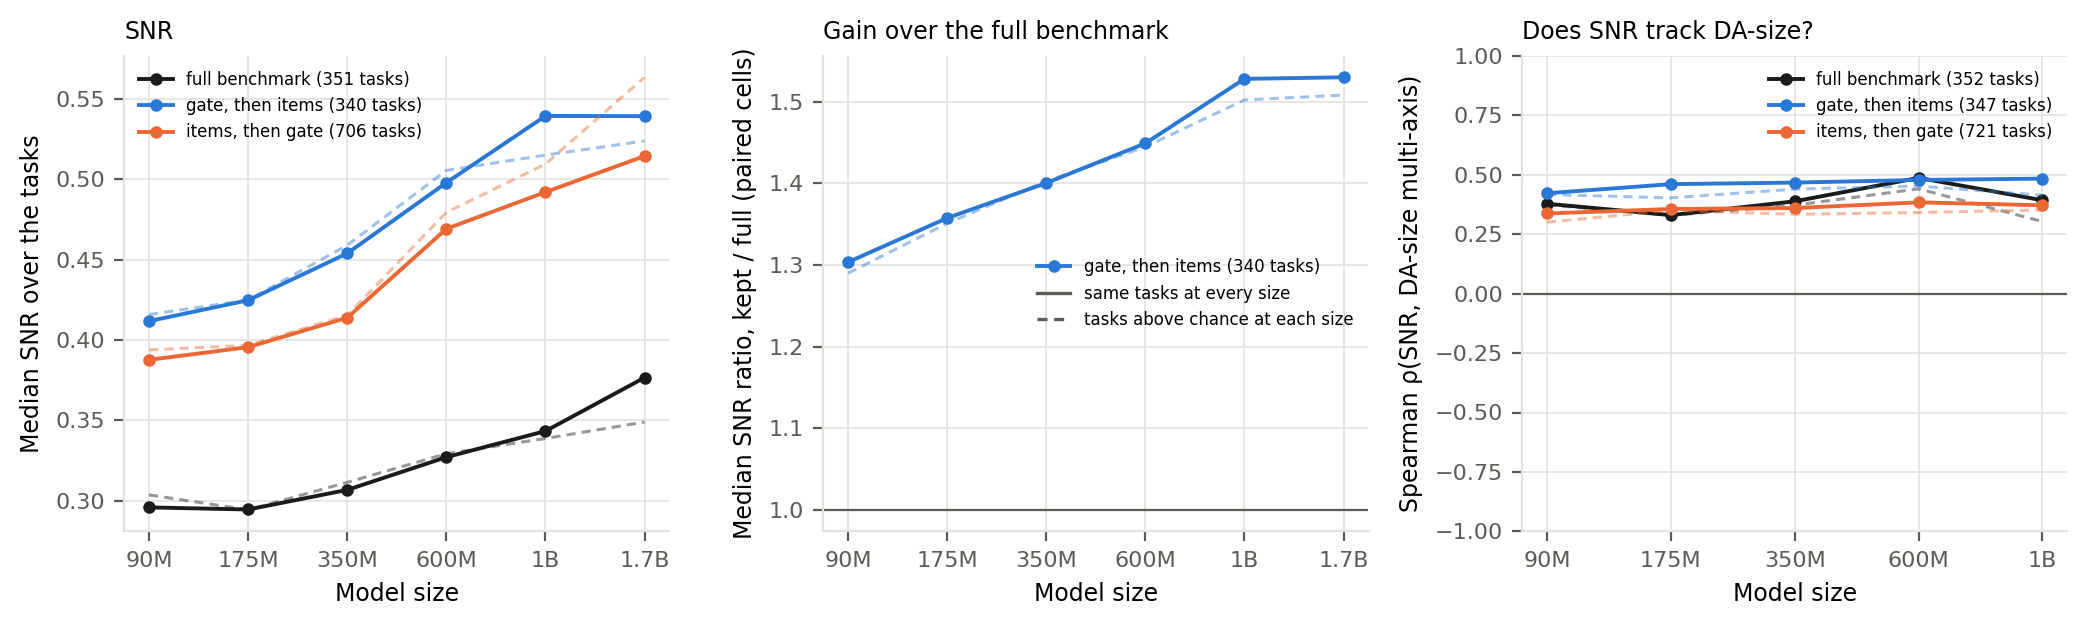
\includegraphics[width=\textwidth,height=0.8\textheight,keepaspectratio]{figures/app_rq12_fixed_above_chance_items.png}
% source: src/signal-and-noise/analysis/rq12_above_chance_items/pretraining/predictivity/above_chance_items_snr_fixed_tasks_paper.png
\caption{\textbf{Holding the tasks fixed moves the median SNR of the items-then-gate ordering by at most $-$0.05 (at 1.7B), so part of the line's movement comes from its changing tasks.} Figure~\ref{fig:app_rq12_above_chance_items} redrawn with one task set per line, the tasks of each ordering that have a value at every point (solid), against the original (dashed). On the 706 tasks with a value at every point, the line reads 0.39 at 90M and 0.51 at 1.7B, against 0.39 and 0.56 on the tasks of each point (757--842).}
\label{fig:app_rq12_fixed_above_chance_items}
\end{figure*}

\begin{figure*}[p]
\centering
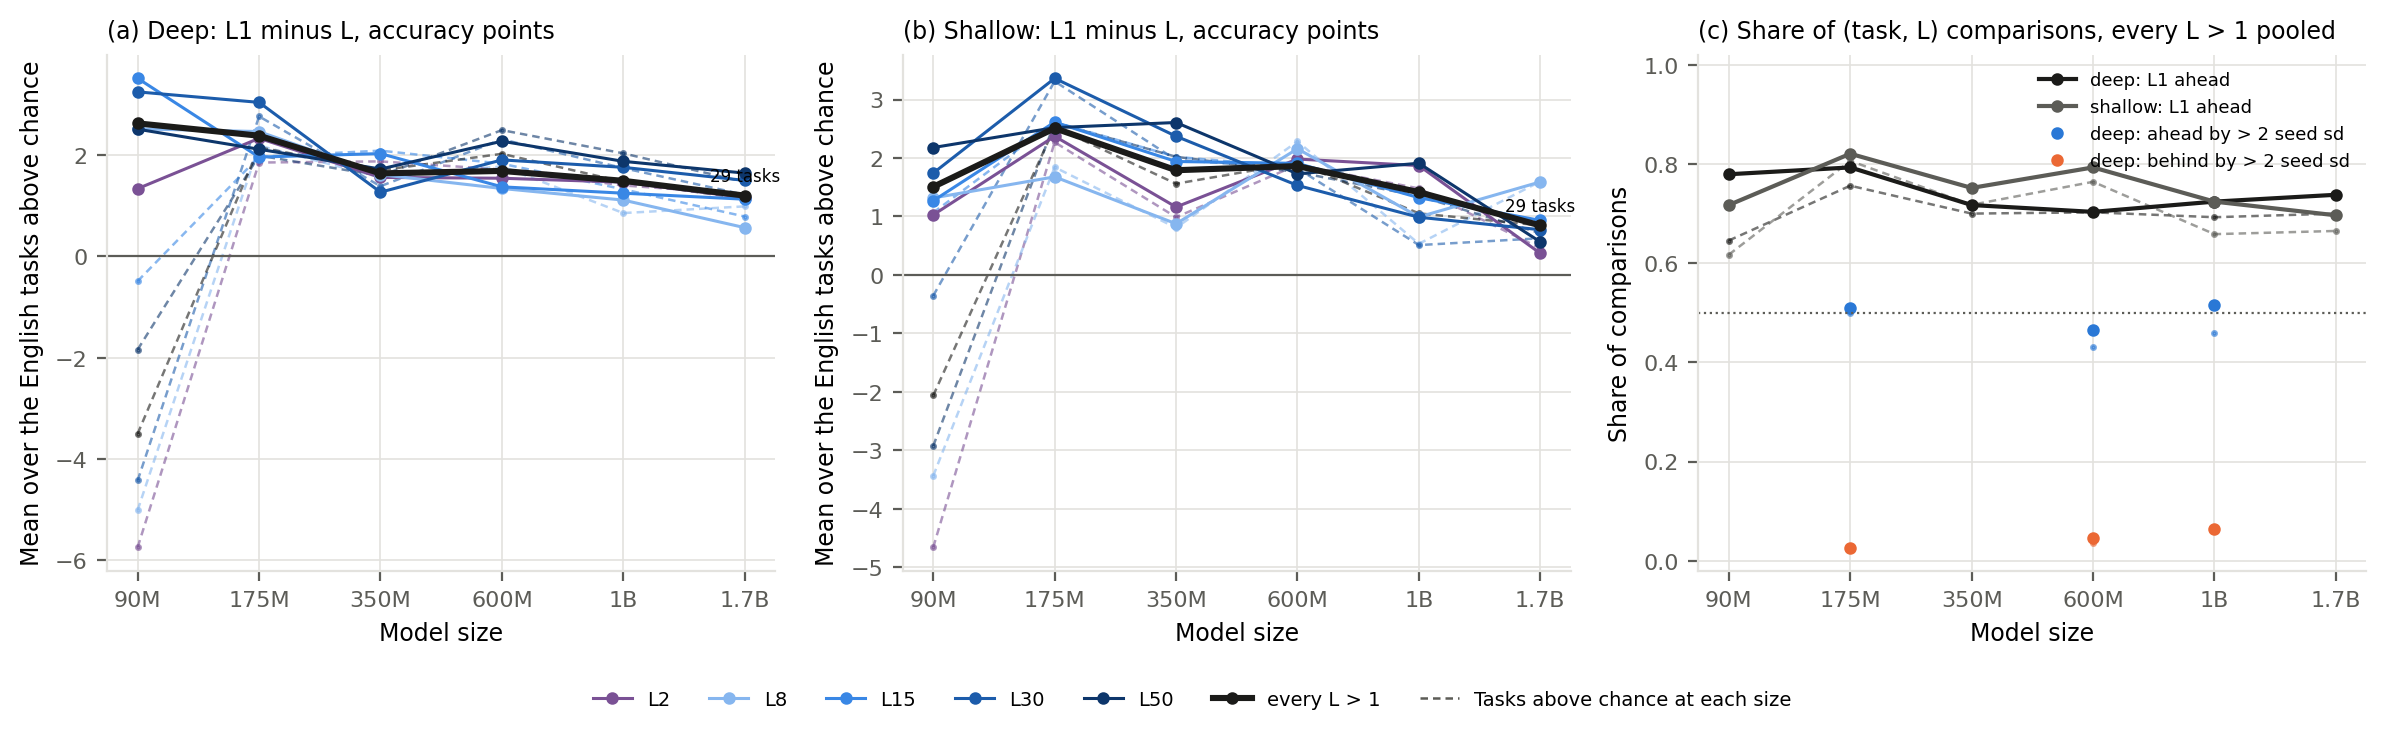
\includegraphics[width=\textwidth,height=0.8\textheight,keepaspectratio]{figures/app_rq13_fixed_english_only.png}
% source: src/signal-and-noise/analysis/rq13_english_only/pretraining/predictivity/english_only_scores_fixed_tasks_paper.png
\caption{\textbf{Holding the tasks fixed moves the deep cells' mean gap in points to every other language setting by at most +6.1 (at 90M), which changes its sign, so the 90M point is a population effect.} Figure~\ref{fig:app_rq13_english_only} redrawn with one task set per line, the English tasks of each comparison that have a value at every point (solid), against the original (dashed). On the 29 tasks with a value at every point, the line reads 2.6 at 90M and 1.2 at 1.7B, against $-$3.5 and 1.1 on the tasks of each point (32--41). Over every line of the panel the largest shift is +7.7 (K30, at 90M).}
\label{fig:app_rq13_fixed_english_only}
\end{figure*}
